\section{All Fresh Controlled Comparison Cases}
\label{app:fresh-evidence-cases}
These are complete configuration blocks from the existing proposal:
28 Cora learning-rate runs and 48 sensing gauge attempts.
The Cora block has 28 complete 1000-epoch runs. The gauge block has
43 complete 1000-update runs and five confirmed nonfinite-objective
failures after the diagnostic replay audit in
Appendix~\ref{app:failure-recovery}. The recovered AdamW run retains
its original diagnostic-stop records and exact optimizer-prefix checks.
Configurations, result records, full epoch trajectories, source hashes,
paired product trajectories, and selection rules are retained.
The task-comparison table uses only validation information to choose
the reported learning rates and checkpoints. This is one seed and
one fixed momentum coefficient, so no confidence-interval or
fully tuned cross-family superiority claim is made.
Shared-machine wall times are retained but are not used as a
speed benchmark.
\begin{table}[t]
\centering\small
\caption{Fresh completed rank-one sensing gauge stress: 12 prescribed gauges per method, 1000 updates each, seed 42. $\Delta_T=\|X_T^{(Q)}-X_T^{(I)}\|_F/\|X_*\|_F$; the maximum uses completed runs, and failed attempts are counted explicitly. $\bar\rho_{\rm upd}$ averages the measured update-direction vertical-energy ratio. Identity error is the final reconstruction error without a gauge perturbation.}
\label{tab:fresh-gauge}
\setlength{\tabcolsep}{4pt}
\begin{tabular}{lrrrr}
\toprule Method & Finished/12 & Max.\ $\Delta_T$ & $\bar\rho_{\rm upd}$ & Identity error\\\midrule
AdamW & 12/12 & $1.07\!\times\!10^{0}$ & $1.35\!\times\!10^{-1}$ & 0.0460\\
SGD-M & 7/12 & $8.86\!\times\!10^{-1}$ & $5.65\!\times\!10^{-5}$ & 0.3797\\
Balance-only & 12/12 & $5.40\!\times\!10^{-5}$ & $1.91\!\times\!10^{-6}$ & 0.9994\\
\rowcolor{oursbg}QuotientOpt & 12/12 & $5.20\!\times\!10^{-5}$ & $1.20\!\times\!10^{-14}$ & 0.9994\\
\bottomrule
\end{tabular}
\end{table}
\begin{table}[t]
\centering\small
\caption{Cora/GCN input adapter, rank 4, seed 42: the complete seven-learning-rate block at $\beta=0.9$, with 1000 epochs per run. Each run uses its earliest maximum-validation-accuracy checkpoint; each method then selects its learning rate by validation accuracy, breaking ties by smaller learning rate. Test metrics do not enter either selection rule; the final 1000-epoch metric is also shown.}
\label{tab:fresh-cora}
\setlength{\tabcolsep}{4pt}
\begin{tabular}{lrrrrr}
\toprule Method & LR & Epoch & Val.\ (\%) & Test sel.\ (\%) & Test 1000 (\%)\\\midrule
AdamW & $10^{-2}$ & 25 & 67.2 & 67.6 & 66.5\\
SGD-M & $10^{-2}$ & 56 & 74.2 & 74.0 & 73.0\\
Balance-only & $10^{-2}$ & 67 & 73.0 & 72.0 & 69.8\\
\rowcolor{oursbg}QuotientOpt & $10^{-2}$ & 67 & 73.0 & 71.9 & 69.8\\
\bottomrule
\end{tabular}
\end{table}

\begin{table}[t]
\centering\small
\renewcommand{\arraystretch}{1.18}\setlength{\tabcolsep}{5pt}
\caption{\textbf{All seven learning rates: Cora validation accuracy (\%).} Rank-4 input adapter, seed 42, 1000 epochs. Each entry is the maximum validation accuracy of its full run; the corresponding CE trajectories are retained in Figure~\ref{fig:all-lr-loss}.}
\label{tab:cora-lr-accuracy}
\begin{tabular}{@{}lrrrrrrr@{}}
\toprule
Method & $1e-05$ & $3e-05$ & $0.0001$ & $0.0003$ & $0.001$ & $0.003$ & $0.01$\\
\midrule
AdamW & 45.2 & 56.0 & 63.4 & 64.4 & 65.6 & 66.2 & 67.2\\
SGD-M & 36.4 & 61.6 & 69.4 & 70.2 & 71.8 & 71.2 & 74.2\\
Balance-only & 36.4 & 61.8 & 69.8 & 70.6 & 71.2 & 71.8 & 73.0\\
\rowcolor{oursbg}\textbf{QuotientOpt} & 36.6 & 61.8 & 69.8 & 70.6 & 71.2 & 71.8 & 73.0\\
\bottomrule
\end{tabular}
\end{table}

\begin{table}[ht]
\centering\small
\caption{Every prescribed sensing gauge. Entries are final $\Delta_T$ relative to the same method at the identity gauge. F denotes a recorded numerical failure; no finite metric is substituted. Scalar values are $q$ in $Q=qI$; dense values are $\kappa(Q)$.}
\label{tab:fresh-gauge-cases}
\begin{tabular}{lrrrrr}
\toprule Gauge & Value & AdamW & SGD-M & Balance & QO\\\midrule
scalar & $10^{-3}$ & $1.07\!\times\!10^{0}$ & \textsf{F} & $1.28\!\times\!10^{-5}$ & $1.41\!\times\!10^{-5}$\\
scalar & $10^{-2}$ & $9.30\!\times\!10^{-1}$ & \textsf{F} & $1.36\!\times\!10^{-5}$ & $1.50\!\times\!10^{-5}$\\
scalar & $10^{-1}$ & $2.68\!\times\!10^{-1}$ & $8.71\!\times\!10^{-1}$ & $1.14\!\times\!10^{-5}$ & $2.03\!\times\!10^{-5}$\\
scalar & $10^{0}$ & 0 & 0 & 0 & 0\\
scalar & $10^{1}$ & $4.47\!\times\!10^{-2}$ & $3.63\!\times\!10^{-1}$ & $1.60\!\times\!10^{-5}$ & $2.35\!\times\!10^{-5}$\\
scalar & $10^{2}$ & $2.99\!\times\!10^{-1}$ & $8.86\!\times\!10^{-1}$ & $1.50\!\times\!10^{-5}$ & $1.97\!\times\!10^{-5}$\\
scalar & $10^{3}$ & $8.86\!\times\!10^{-1}$ & \textsf{F} & $1.72\!\times\!10^{-5}$ & $1.98\!\times\!10^{-5}$\\
dense & $10^{0}$ & $2.82\!\times\!10^{-2}$ & $5.62\!\times\!10^{-7}$ & $1.79\!\times\!10^{-5}$ & $2.14\!\times\!10^{-5}$\\
dense & $10^{1}$ & $3.48\!\times\!10^{-2}$ & $2.67\!\times\!10^{-1}$ & $1.46\!\times\!10^{-5}$ & $1.55\!\times\!10^{-5}$\\
dense & $10^{2}$ & $6.88\!\times\!10^{-2}$ & $2.92\!\times\!10^{-1}$ & $2.47\!\times\!10^{-5}$ & $2.40\!\times\!10^{-5}$\\
dense & $10^{3}$ & $2.47\!\times\!10^{-1}$ & \textsf{F} & $2.44\!\times\!10^{-5}$ & $2.88\!\times\!10^{-5}$\\
dense & $10^{4}$ & $9.35\!\times\!10^{-1}$ & \textsf{F} & $5.40\!\times\!10^{-5}$ & $5.20\!\times\!10^{-5}$\\
\bottomrule
\end{tabular}
\end{table}
\begin{table}[ht]
\centering\small
\caption{All Cora learning rates in the fixed block. Entries are test accuracies (\%) at the checkpoint chosen using that run's validation accuracy, not at a test-selected checkpoint.}
\label{tab:fresh-cora-all}
\begin{tabular}{rrrrr}
\toprule LR & AdamW & SGD-M & Balance & QO\\\midrule
$10^{-5}$ & 44.9 & 40.0 & 40.0 & 40.0\\
$3\times10^{-5}$ & 59.9 & 62.1 & 62.2 & 62.1\\
$10^{-4}$ & 63.0 & 71.3 & 71.1 & 71.3\\
$3\times10^{-4}$ & 64.9 & 71.6 & 71.4 & 71.4\\
$10^{-3}$ & 66.5 & 70.4 & 70.1 & 70.1\\
$3\times10^{-3}$ & 66.1 & 71.9 & 70.3 & 70.3\\
$10^{-2}$ & 67.6 & 74.0 & 72.0 & 71.9\\
\bottomrule
\end{tabular}
\end{table}

\begin{table}[ht]
\centering\small
\caption{Secondary loss-based early stopping on the same 28 Cora runs. Select the lowest validation cross-entropy over epochs and learning rates; ties use smaller LR, then earlier epoch. This is distinct from the primary validation-accuracy criterion in Table~\ref{tab:fresh-cora}. Test loss is read at the validation-selected checkpoint and is not minimized during selection.}
\label{tab:secondary-ce}
\begin{tabular}{lrrrrr}
\toprule Method & LR & Epoch & Val.\ CE & Test CE & Test acc.\ (\%)\\\midrule
AdamW & $10^{-2}$ & 15 & 1.1728 & 1.0525 & 64.7\\
SGD-M & $10^{-2}$ & 36 & 0.9079 & 0.8579 & 73.1\\
Balance-only & $10^{-2}$ & 37 & 0.9261 & 0.8730 & 72.0\\
\rowcolor{oursbg}QuotientOpt & $10^{-2}$ & 37 & 0.9261 & 0.8730 & 72.0\\
\bottomrule
\end{tabular}
\end{table}

\begin{figure}[ht]
\centering
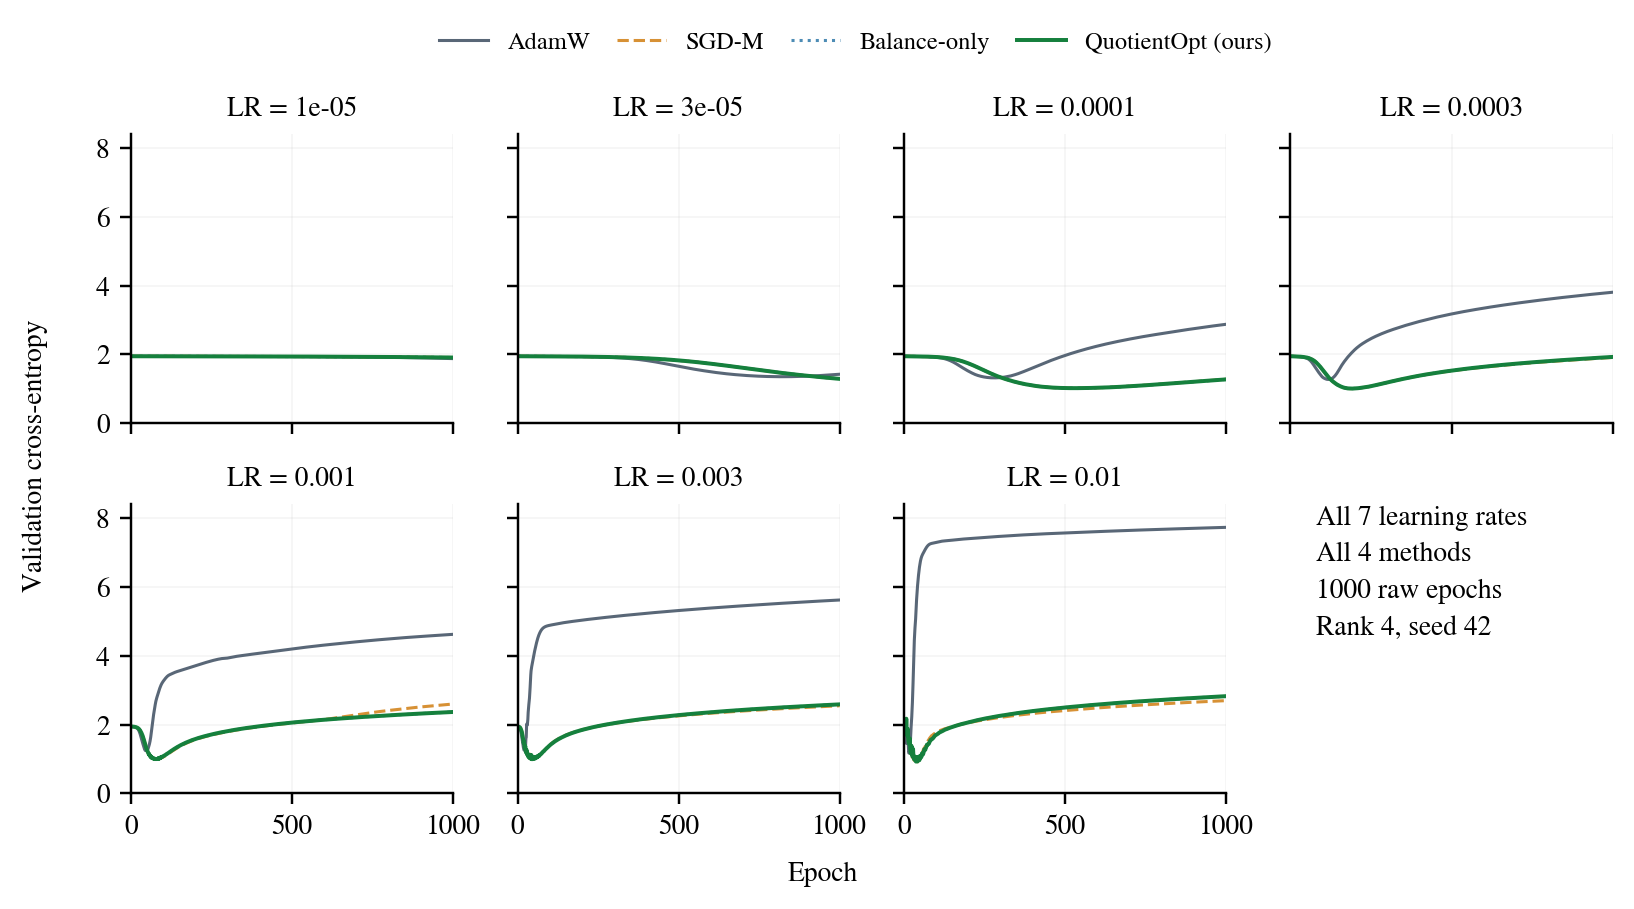
\includegraphics[width=.99\linewidth]{figures/cora_all_lr_loss.png}
\caption{Every learning rate in the complete Cora/GCN input-adapter
block: rank 4, seed 42, $\beta=0.9$. All four methods and all 1000
raw epoch observations are retained, with common axes, no smoothing,
and no omitted learning rates. This figure supplies the full learning-rate
context for the accuracy-selected core loss curves in
Figure~\ref{fig:core-loss}.}
\label{fig:all-lr-loss}
\end{figure}
